\chapter[Sprint 2]{Study and Implementation of Sprint 2: Project Management}

\section{Introduction}

Sprint 2 implements comprehensive project management functionality within the UML diagram platform. This sprint introduces essential features enabling users to organize, manage, and maintain UML projects effectively, serving as the foundation for user workflow organization with capabilities for project creation, modification, visualization, and data export.

\section{Sprint Planning}

\subsection{Objectives}
Sprint 2 aims to implement a complete project management system allowing users to efficiently organize UML diagram projects through:
\begin{itemize}
    \item Project creation with customizable parameters
    \item Intuitive project browsing and viewing capabilities
    \item Secure project modification features
    \item Safe project deletion with confirmations
    \item Robust export system for compressed project diagrams
\end{itemize}

\subsection{Sprint Backlog}


\begin{longtable}{|c|l|c|p{8cm}|c|}
    \caption{Manage Projects User Stories Requirements Table} \label{tab:manage_projects} \\
    \hline
    \textbf{ID} & \textbf{Feature} & \textbf{Sub-ID} & \textbf{User Story} & \textbf{Priority} \\
    \hline
    \endfirsthead
    
    \multicolumn{5}{c}%
    {{\bfseries \tablename\ \thetable{} -- continued from previous page}} \\
    \hline
    \textbf{ID} & \textbf{Feature} & \textbf{Sub-ID} & \textbf{User Story} & \textbf{Priority} \\
    \hline
    \endhead
    
    \hline \multicolumn{5}{|r|}{{Continued on next page}} \\ \hline
    \endfoot
    
    \hline
    \endlastfoot
    
    3 & Manage Projects & 3.1 & As a user; I want to create a new project so that I can organize my diagrams. & M \\
    \hline
      &  & 3.2 & As a user; I want to view my project details. & M \\
    \hline
      &  & 3.3 & As a user; I want to update project details. & M \\
    \hline
      &  & 3.4 & As a user; I want to delete a project. & M \\
    \hline
      &  & 3.5 & As a user; I want to download project diagrams as images in a compressed ZIP file. & S \\
    \hline
      &  & 3.6 & As a user; I want to share my project with others. & S \\
    \hline
    \end{longtable}
\section{Analysis and Design}

\subsection{Use Case Analysis}

\begin{figure}[H]
\centering
\includegraphics[width=0.75\textwidth]{conception/SprintIII/use_case_diagrams/use_case_diagram_of_SprintIII.png}
\caption{Sprint 2 Use Case Diagram}
\label{fig:use_case_sprint3}
\end{figure}

\begin{figure}[H]
\centering
\includegraphics[width=0.8\textwidth]{conception/SprintIII/use_case_diagrams/refined_use_case_feature_project_management.png}
\caption{Refined Project Management Use Cases}
\label{fig:refined_use_case_project_mgmt}
\end{figure}

\subsection{Key Use Case Specifications}

\subsubsection{Create New Project (UC-3.1)}
\textbf{Main Flow}: User accesses creation form → enters project details → selects type/settings → system validates → creates project → displays confirmation → redirects to dashboard.

\textbf{Alternative Flows}: Invalid input triggers validation errors; system errors maintain form data.

\subsubsection{View Project (UC-3.2)}
\textbf{Main Flow}: User accesses project list → selects project → system retrieves details → displays organized layout → enables diagram navigation.

\textbf{Alternative Flows}: Empty projects show appropriate messages; access errors redirect or show permissions.

\subsubsection{Update Project (UC-3.3)}
\textbf{Main Flow}: User accesses edit interface → modifies fields → submits changes → system validates → saves to database → confirms success.

\textbf{Alternative Flows}: No changes or validation errors handled appropriately.

\subsubsection{Delete Project (UC-3.4)}
\textbf{Main Flow}: User selects deletion → system shows confirmation → user confirms → system removes data → cleans resources → confirms deletion.

\textbf{Alternative Flows}: Cancellation or shared project warnings handled safely.

\subsubsection{Download Compressed (UC-3.5)}
\textbf{Main Flow}: User accesses export → selects formats → initiates download → system generates diagrams → creates zip → downloads file.

\textbf{Alternative Flows}: Large projects show progress; selective export options available.


\section{Sequence Diagrams}

The following diagrams illustrate system component interactions:

\begin{figure}[H]
\centering
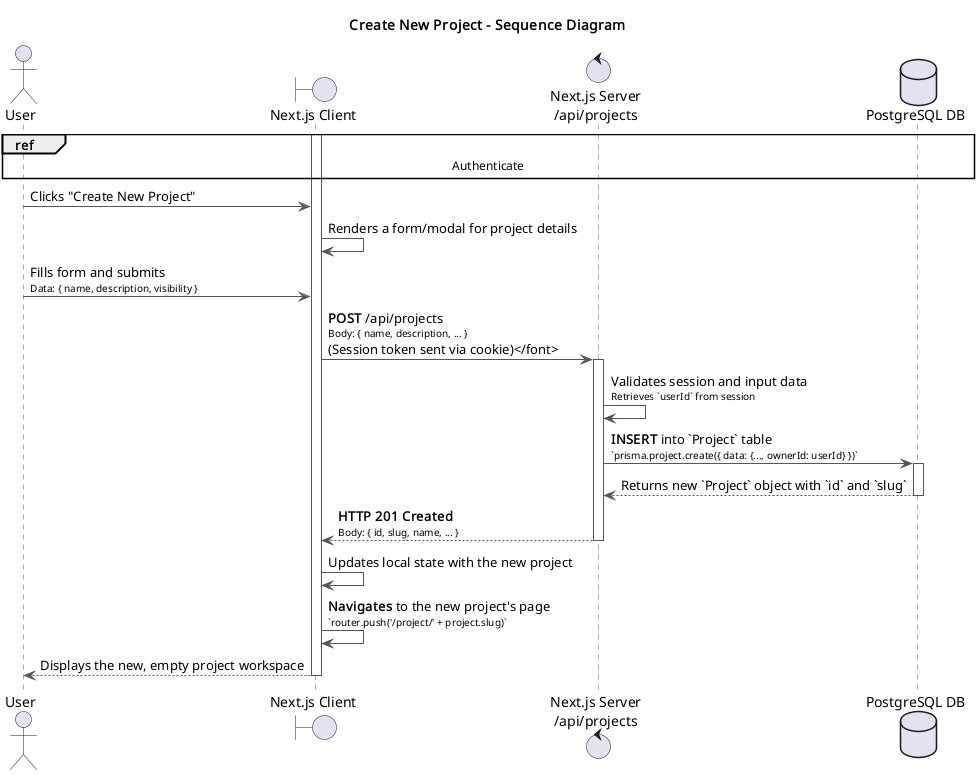
\includegraphics[width=1\textwidth]{conception/SprintIII/sequence_diagrams/sequence_projectManagement_3_1_CreateNewProject.png}
\caption{Create Project Sequence}
\label{fig:seq_create_project}
\end{figure}

\begin{figure}[H]
\centering
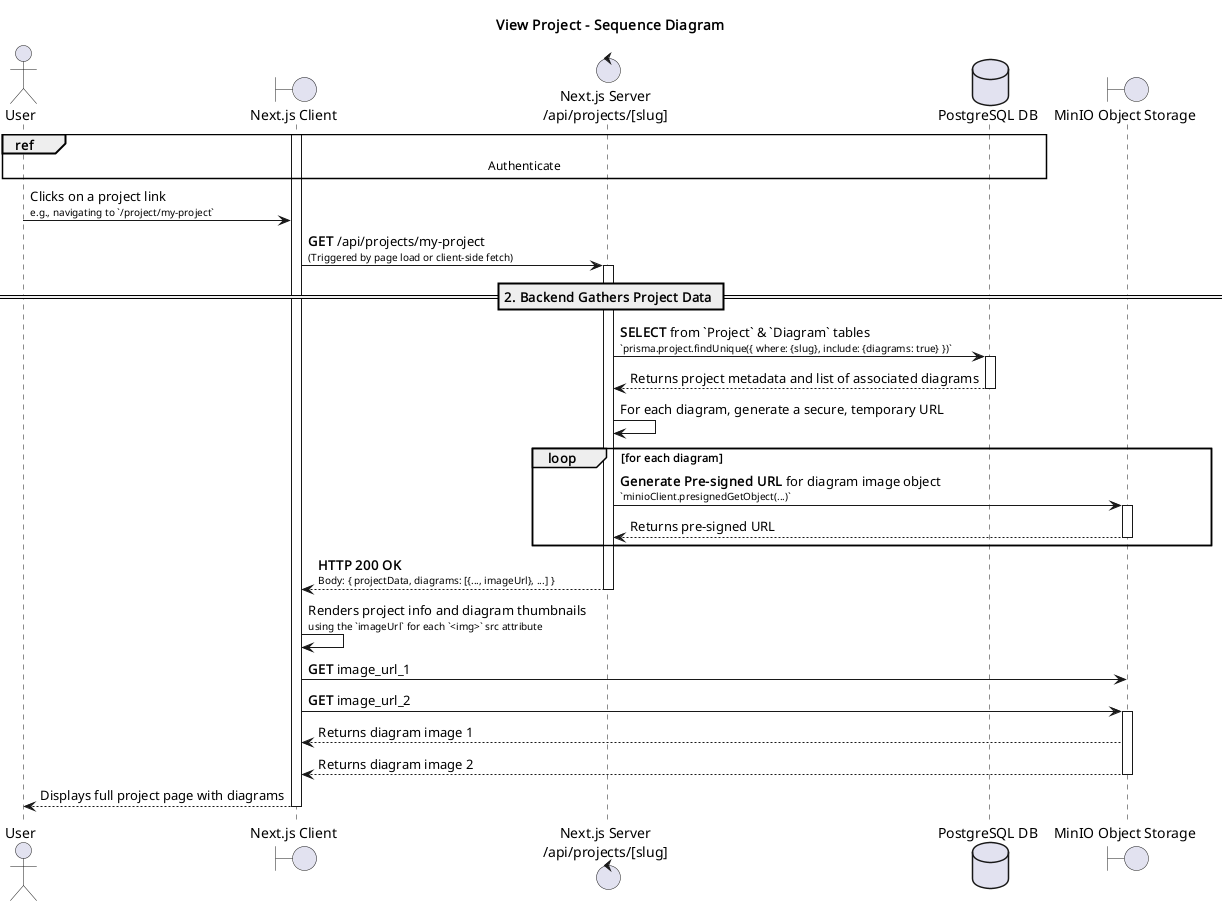
\includegraphics[width=1\textwidth]{conception/SprintIII/sequence_diagrams/sequence_projectManagement_3_2_ViewProjectDetails.png}
\caption{View Project Sequence}
\label{fig:seq_view_project}
\end{figure}

\begin{figure}[H]
\centering
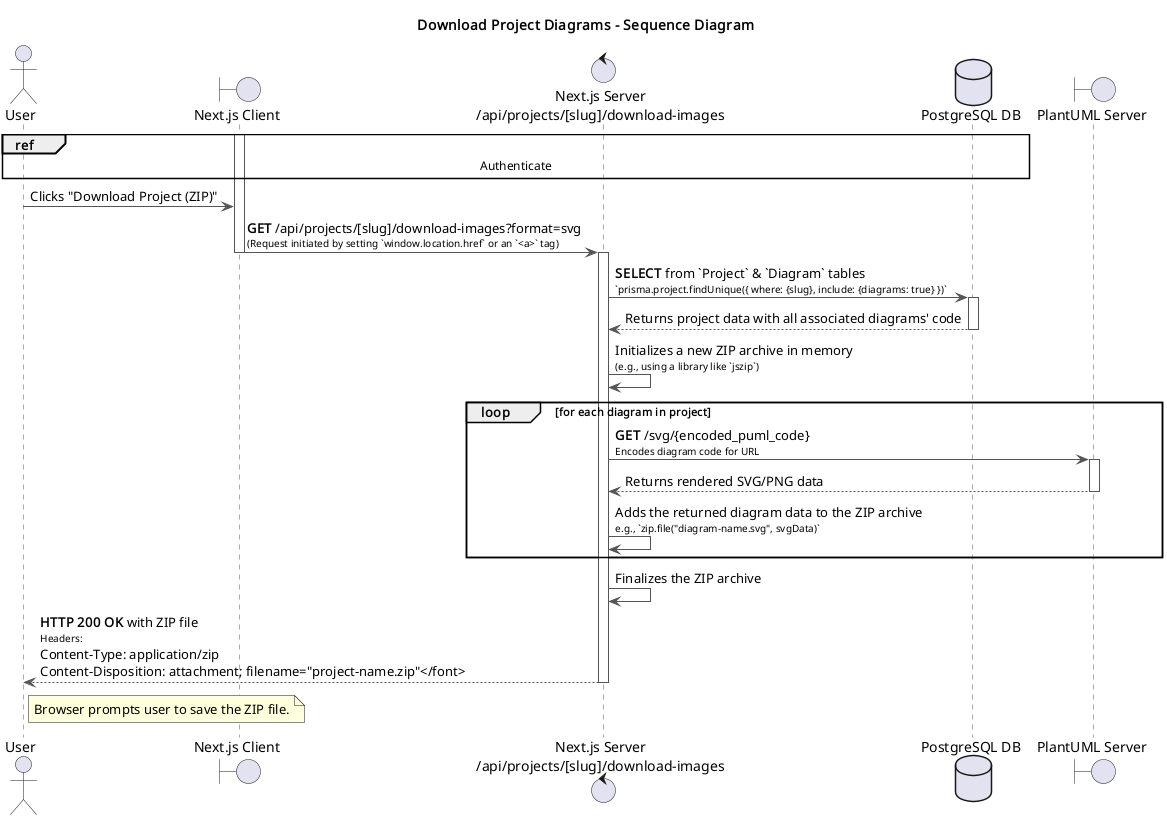
\includegraphics[width=1\textwidth]{conception/SprintIII/sequence_diagrams/sequence_projectManagement_3_5_DownloadProjectDiagramsAsZip.png}
\caption{Download Project Diagrams Sequence}
\label{fig:seq_download_project}
\end{figure}

\section{Implementation Results}

\subsection{User Interface Screenshots}

\begin{figure}[H]
\centering
\includegraphics[width=0.6\textwidth]{screenshots/home.png}
\caption{Home page with project overview}
\label{fig:home_page}
\end{figure}

\begin{figure}[H]
\centering
\includegraphics[width=0.7\textwidth]{screenshots/add-project.png}
\caption{Project creation interface}
\label{fig:add_project}
\end{figure}

\begin{figure}[H]
\centering
\includegraphics[width=0.7\textwidth]{screenshots/project-page.png}
\caption{Project details and management}
\label{fig:project_page}
\end{figure}


\section{Sprint Retrospective}

\subsection{Achievements}
\begin{itemize}
    \item Complete CRUD operations implementation
    \item Robust export functionality with multiple formats
    \item Intuitive user interfaces with validation
    \item Strong technical execution and requirement analysis
\end{itemize}

\subsection{Areas for Improvement}
\begin{itemize}
    \item Enhanced error handling mechanisms
    \item Performance optimization for large projects
    \item Extended sharing capabilities
\end{itemize}

\section{Conclusion}

Sprint 2 established a robust project management foundation providing users with comprehensive tools for organizing and managing UML projects effectively. The implemented features deliver significant value through intuitive interfaces, reliable functionality, and scalable architecture. This sprint positions the platform for continued growth and enhanced collaboration capabilities, demonstrating the team's ability to deliver complex functionality while maintaining high quality standards.